% !TeX root = ../main.tex

\chapter{基于区间算数的整数缺陷检测}

{\color{red} 抽取后的重写}

本章提出基于区间算数的整数缺陷检测技术,借助组合静态分析框架,在程序局部进行高精度的区间分析,对整体使用高效率的算法对各个局部分析结果进行组合,从而实现高效的C语言整数缺陷检测。本章的工作对提升现有工具的整数缺陷分析的精度和效率具有重要意义。

\section{引言}

若要判定程序中整型变量所参与的计算是否可能产生整型溢出、除零异常及缓冲区溢出等缺陷,传统的解决方案是使用抽象解释将程序中的整型变量上近似抽象为1个整数区间。结合数据流分析,得到整型变量在整数区间抽象域上的近似值,并以此判定整型变量的操作是否安全。

尽管该方法能够在简单逻辑代码上得到较好的分析效果,但由于抽象域的表示能力有限,在程序的逻辑分支复杂的情况下,因状态合并操作所带来的精度损失较大,通常经过数次操作即到达抽象域的上界。

\begin{figure}[htb]
	\begin{subfigure}[b]{.5\linewidth}
			\begin{lstlisting}[xleftmargin=.15\textwidth]
void funcA(int i) {
	int x;
	if (i > 0) {
		x = funcB(i) - 5;
	} else {
		x = 5 - funcB(i);
	}
	assert(x != 0);
}
			\end{lstlisting}
%			\caption{A listing}
	\end{subfigure}
	\begin{subfigure}[b]{.5\linewidth}
			\begin{lstlisting}[xleftmargin=.25\textwidth]
int funcB(int i) {
	int x;
	if (x > 3) {
		x = 3 - i;
	} else {
		x = i;
	}
	return x;
}
			\end{lstlisting}
%		   (-∞, 3]
%			\caption{A listing}
\end{subfigure}
	\caption{基于区间算数的缺陷检测方法举例}
	\label{fig:codeExampleForSignRange}
\end{figure}{\tiny }

考虑图\ref{fig:codeExampleForSignRange}所示代码:函数A作为程序的入口,通过用户输入得到整型数值i,并根据i的大小使用不同的逻辑调用函数B并处理函数返回值。这里为讨论方便起见,规定int可表示所有整数值。若使用传统的基于整数区间抽象的数据流分析算法进行程序分析,易知函数B的返回值范围是$ [-\infty, 3] $,则函数A中第4行x的取值范围是$ [-\infty, -2] $,第6行x的取值范围是$ [2, +\infty] $。在第8行,由于状态合并,x的取值范围是$ [-\infty, +\infty] $,这将导致目标属性不成立。但实际上x的取值范围不包含0,目标属性是安全的。

为了解决上述问题,进一步提高程序分析的精度,本章提出了基于区间算数的整数缺陷检测技术,并在基于CPAchecker\cite{beyer2007configurable}的可配置的组合静态分析工具Tsmart上进行了实现。经过实验,基于本章工作实现的工具在Juliet测试集上的误报率小于3\%,漏报率为0\%。

\section{预备知识}

%\subsection{静态分析}
%
%静态分析是指在不运行代码的情况下,对程序源代码进行行为分析,从而判定程序是否满足某种特性。在代码的审查与优化、代码的缺陷分析与修复等方面有着大量应用。衡量静态分析技术的优劣通常考虑两个方面:分析精度和分析效率。分析精度用于衡量程序的实际行为与分析结果之间的匹配程度,分析效率则注重程序分析所消耗的资源大小,包括时间、存储的开销等。通常,程序分析的精度与效率是不可兼得的:分析精度的提高往往伴随着分析效率的下降,在实际应用中,我们往往需要平衡静态分析的精度与资源消耗,在不占用太多的资源下获得较好的分析精度一直是静态分析领域所重点关注的问题之一。

\subsection{控制流自动机}
\label{sec:控制流自动机}

控制流自动机(Control-flow Automaton,CFA)是命令式程序的一种语义等价表示方法,它是一个有向图:
\begin{definition}
	CFA可表示为有向图$ G = (N, E) $:$ N $是节点的集合,节点$ n \in N $表示程序的状态。$ E \subseteq N \times Ops \times N $是边的集合,有向边$ e = (n, op, n') \in E $表示从某个程序状态到下一个程序状态的过程,其中,$ Ops $是状态之间所执行的指令。一般地,我们用$ pred(e) $表示边$ e $的前驱节点$ n $,用$ succ(e) $表示边$ e $的后继节点$ n' $,用$ act(e) $表示边$ e $所执行的动作$ op $。
\end{definition}

在本文中,若无特殊说明,CFA是LLVM-IR语言上的等价表示,有向边$ e $根据其表示的指令的不同,可分为如下几类:
\begin{itemize}
	\item 空白边(BlankEdge):表示没有执行动作的边。即$ act(e) = \varepsilon $;
	
	\item 假设边(AssumeEdge):描述了假设条件是否成立。操作$ act(e) = (\%cmp, truth) $,其中$ \%cmp $为条件变量,它对应于LLVM-IR中i1类型的变量,表示假设条件。$ truth \in \{0, 1\}$为条件取值,表示当前边上假设条件变量$ \%cmp $的具体取值。一般地,我们用$ cond(e) $表示假设边的条件变量$ \%cmp $,用$ truth(e) $表示条件变量的取值$ truth $。
	
	\item Phi边(PhiEdge):描述了LLVM-IR中的phi指令。操作$ act(e) = (\%phi, index) $,其中$ \%phi $对应于phi指令,$ index $指示phi边上的第几个操作数作为当前指令的返回结果。
	
	\item 指令边(InstructionEdge):是CFA中最常见的边,描述了当前边执行了一条LLVM-IR指令。操作$ act(e) = (\%inst) $,其中$ \%inst $为所执行的指令。
	
%	\item 函数摘要边(FunctionSummaryEdge)

%	\item 函数调用边与函数返回边(FunctionCallEdge, FunctionReturnEdge):
\end{itemize}

为了便于描述,定义函数$ type $用于获取边的类型:
\begin{align}{\label{align:edgeType}}
	type(e) := \begin{cases}
		blank & e \in BlankEdge\\
		assume & e \in AssumeEdge\\
		phi & e \in PhiEdge\\
		inst & e \in InstructionEdge
	\end{cases}
\end{align}

\subsection{可配置程序分析框架} 

可配置程序分析(Configurable Program Analysis,CPA)是一种通用的程序分析框架,通过设计并配置相关参数,实现在同一框架下完成多种不同的静态分析任务。通常,CPA框架将程序源代码转化为语义等价的控制流自动机并在CFA上多次应用静态分析算法实现程序分析。其中,CFA是源程序的等价表示,可描述为有向图。其节点表示指令位置、边表示控制流操作,如变量声明、运算、赋值、函数调用等。在分析时,我们常将内存地址抽象为内存位置,如访问路径\cite{cheng2000modular}等。

CPA算法的一次分析可表示为四元组$ \mathbb{D} = (D, \rightsquigarrow, merge, stop) $。其中,$ D $为抽象域;$ \rightsquigarrow $为转移关系,规定了在不同的控制流操作下,给定的抽象状态如何转移到新的抽象状态;$ merge $为状态合并算子;$ stop $为状态覆盖算子。

算法\ref{alg:CPA算法}描述了CPA的算法流程:算法以分析$ \mathbb{D}$、CFA图$ G $和初始状态$ e_0 \in E $作为输入,通过维护工作队列$ waitlist $和可达状态集$ R $并根据转移关系$ \rightsquigarrow $来计算当前状态$ e $的后继状态。工作队列和可达集的维护算法如算法\ref{alg:UpdateRW}所示,对每个后继状态$ e' $使用$ merge $算子来更新所有可达状态,如果可达状态$ e'' $被更新,则将该状态加入到等待队列$ waitlist $中以更新其后继状态。如果更新后的可达状态无法覆盖$ e' $,则将该状态分别加入$ waitlist $和可达集中。

\begin{breakablealgorithm}
	\caption{CPA算法}
	\label{alg:CPA算法}
	\begin{algorithmic}[1]
		
		\Require $ \mathbb{D} = (D, \rightsquigarrow, merge, stop) $,CFA图$ G $,初始状态$ e_0 \in E $
		\Ensure 可达状态集$ R $
		
		\State $ waitlist \gets \left\{ e_0 \right\} , R \gets \left\{ e_0 \right\}$
		\While{$ waitlist \ne \emptyset $}
			\State 取出$ waitlist $的首元素$ e $;
			\ForAll{$ e' $满足$ e \rightsquigarrow e' $}
				\State \Call{UpdateRW}{$ e', R, waitlist, merge, stop $};
			\EndFor
		\EndWhile
		
	\end{algorithmic}
\end{breakablealgorithm}

\begin{breakablealgorithm}
	\caption{UpdateRW算法}
	\label{alg:UpdateRW}
	\begin{algorithmic}[1]
		
		\Function{UpdateRW}{$ e', R, waitlist, merge, stop $}
			\ForAll{$ e' \in R $}
				\State $ e_{new}  \gets merge(e, e')$;
				\If{$ e_{new} \ne e' $}
					\State $ waitlist \gets (waitlist \cup \{e_{new}\}) \setminus \{e'\} $;
					\State $ R \gets (R \cup \{e_{new}\}) \setminus \{e'\} $;
				\EndIf
			\EndFor
			\If{$\neg stop(e, R)$}
				\State $ waitlist \gets (waitlist \cup \{e\}) $;
				\State $ R \gets R \cup \{e\} $;
			\EndIf
		\EndFunction
		
	\end{algorithmic}
\end{breakablealgorithm}

\section{基于线性空间的抽象域设计}

本节介绍基于线性空间的抽象域,抽象域的组成结构如图\ref{fig:Domains}所示。RangeState为程序变量在线性空间的抽象表示,它包含整型变量的访问路径、取值范围、符号等信息。

\begin{figure}[H]
	\centering
	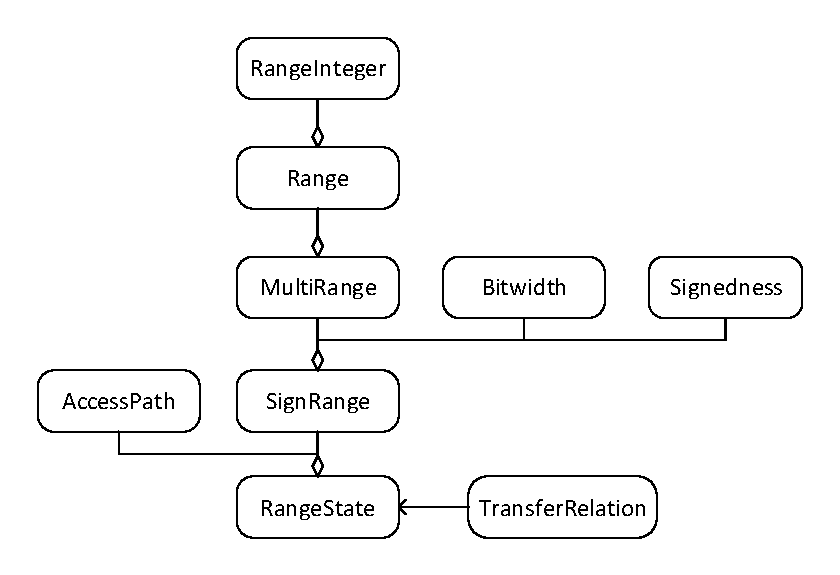
\includegraphics{Domains.pdf}
	\caption{抽象域的组成}
	\label{fig:Domains}
\end{figure}

\subsection{扩展的整数(RangeInteger)理论域}
\label{sec:Integer}

整型变量的可能取值是一个整数的集合,在这里我们使用扩展的整数RangeInteger来表示一个具体的整数,它是整数域$ \mathbf{Z} $的一个拓展。

\begin{definition}
	记$ D_I := \mathbf{Z} \cup \{ +\infty, -\infty, arb, nan\}  $为扩展的整数理论域。
	\begin{itemize}
		\item $ D_I $上的最大元($ \top_I $)为$ arb $,它表示任意值;最小元($ \bot_I $)为$ nan $,它表示非数;
		
		\item $ D_I $上的偏序关系($ \le_I $)为$ \mathbf{Z} $上的自然扩展,对于元素$ -\infty $与$ +\infty $,规定$ -\infty < +\infty $,且对任意$ x \in \mathbf{Z} $,有$ x < +\infty $以及$ -\infty < x $。特殊地,$ -\infty $与$ -\infty $、$ +\infty $与$ +\infty $无法比较,$ \bot_I, \top_I $与其他任意元素无法比较。
		
		\item $ D_I $上的上确界操作($ \sqcup_I $)定义为:\\
		\centerline{$ a \sqcup_I b := \begin{cases}
			\top_I & a \ne \bot_I \land b \ne \bot_I\\
			a & b = \bot_I\\
			b & a = \bot_I\\
			\bot_I & a = \bot_I \land b = \bot_I
			\end{cases} $}
	\end{itemize}
\end{definition}

对于元素$ -\infty $或$ +\infty $参与的运算,其规则如表\ref{tab:RangeInteger运算规则}所示。其中,函数$ signum $为取符号数,具体定义如下:
\begin{align}
	signum(x) := \begin{cases}
		1 & (x \in \mathbf{Z} \land x > 0) \lor x = +\infty\\
		0 & x = 0\\
		-1 & (x \in \mathbf{Z} \land x < 0) \lor x = -\infty
	\end{cases}
\end{align}

特别的,元素$ +\infty $与$ -\infty $所参与的某些运算是未定义的。这样的运算在表中记录为$ nan $,如$ (+\infty) +_I (-\infty), (+\infty) \div_I (+\infty)  $等。

\begin{longtable}{cclc}
	\caption[RangeInteger运算规则]{RangeInteger运算规则}
	\label{tab:RangeInteger运算规则}  \\ % add \\ command to tell LaTeX to start a new line	
	
	% Appear table header at the first page as well
	\toprule[1.5pt]	
	{\heiti 运算} & {\heiti 符号} & \multicolumn{1}{c}{\heiti 运算规则} \\
	\midrule[1pt]
	\endfirsthead
	
	% Appear the table header at the top of every page
	\multicolumn{3}{c}{续表~\thetable\hskip1em RangeInteger运算规则}\\
	\toprule[1.5pt]	
	{\heiti 运算} & {\heiti 符号} & \multicolumn{1}{c}{\heiti 运算规则} \\
	\midrule[1pt]
	\endhead 
	
	% Appear \hline at the bottom of every page
	\hline
	\multicolumn{3}{r}{续下页}
	\endfoot 
	\endlastfoot
	
	% data begins here				
		negate & $ neg_I $ & $  neg_I(x) :=  \begin{cases}
			-x & x \ne \pm\infty\\
			-\infty & x = +\infty\\
			+\infty & x = -\infty\\
		\end{cases}$\\
		
		add &$  +_I $ & $ x +_I y :=  \begin{cases}
			x + y & x, y \ne \pm\infty\\
			x & x = \pm\infty \land y \ne \pm\infty\\
			y & x \ne \pm\infty \land y = \pm\infty\\
			x & x, y = \pm\infty \land signum(x) = signum(y) \\
			nan & \text{other cases}
		\end{cases}$ \\
		
		subtract & $ -_I $ & $ x -_I y := \begin{cases}
			x - y & x, y \ne \pm\infty\\
			x & x = \pm\infty \land y \ne \pm\infty\\
			neg(y) & x \ne \pm\infty \land y = \pm\infty\\
			x & x, y = \pm\infty \land signum(x) \ne signum(y) \\
			nan & \text{other cases}
		\end{cases} $\\
		
		multiply & $ \times_I $ & $ x \times_I y := \begin{cases}
			x \times y & x, y \ne \pm\infty\\
			+\infty & signum(x) \times signum(y) > 0\\
			-\infty & signum(x) \times signum(y) < 0\\
			nan & \text{other cases}
		\end{cases} $\\
		
		\begin{tabular}{c}
			divide\\
			$ (y \ne 0) $\\
		\end{tabular} & $ \div_I $ & $ x \div_I y := \begin{cases}
			x \div y & x, y \ne \pm\infty\\
			0 & x \ne \pm\infty \land y = \pm\infty\\
			+\infty \times_I signum(x \times_I y) & x = \pm\infty \land y \ne \pm\infty\\				
			nan & \text{other cases}
		\end{cases} $\\
		
		\begin{tabular}{c}
			modular\\
			$ (y > 0) $\\
		\end{tabular} & $ mod_I $ & $ x \mod_I y := \begin{cases}
		x \mod y & x, y \ne \pm\infty\\
		x & x \ge 0 \land y = +\infty\\
		y & x < 0 \land y =+\infty\\
		nan & \text{other cases}
		\end{cases} $\\
		
		\begin{tabular}{c}
			and\\
			or\\
			xor\\
			shl\\
			shr
		\end{tabular} & \begin{tabular}{c}
		$ and_I $\\
		$ or_I $\\
		$ xor_I $\\
		$ <<_I $\\
		$ >>_I $
	\end{tabular} & $ x \cdot_{op_I} y := \begin{cases}
		x \cdot_{op} y & x, y \ne \pm\infty\\
		nan & \text{other cases}
		\end{cases} $\\
	
	% more data here
	\bottomrule[1.5pt]
\end{longtable}

\subsection{线性区间(Range)理论域}
\label{sec:Range}

线性区间Range一个整数区间,表示整型变量的可能取值范围,它是由两个整数$ x, y $构成的二元组。这里,$ x, y $为扩展的整数域RangeInteger上的元素,其定义与偏序关系定义如下。

\begin{definition}
	线性区间理论域$ D_R :=  \{ [x, y] | x \in \mathbf{I}, y \in \mathbf{I}, x \le y \} \cup \{ \emptyset \}$是一个半格:	
	\begin{itemize}
		\item $ D_R $上的最大元($ \top_R $)是$ [-\infty, +\infty] $,最小元($ \bot_R $)是空集$ \emptyset $;
		\item $ D_R $上的偏序关系($ \le_R $)定义为:\\	
		\centerline{$ [x_1, y_1] \le_R [x_2, y_2] \iff x_2 \le x_1 \land y_1 \le y_2 $;}
		\item $ D_R $上的上确界操作($ \sqcup_R $)定义为:\\	
		\centerline{$ [x_1, y_1] \sqcup_R [x_2, y_2] := [\min(x_1, x_2), \max(y_1, y_2)] $,}  \\
		此处$ \max $和$ \min $为$ D_I $上的自然扩展。
	\end{itemize}
\end{definition}

我们在Range上定义一些基础的运算操作,其运算规则如表\ref{tab:Range运算规则}所示。值得注意的是,最小元$ \bot_R $与任何元素的计算结果均为$ \bot_R $,为表示方便,在表中默认操作数均不为$ \bot_R $。

\begin{longtable}{cclc}
	\caption[Range运算规则]{Range运算规则}
	\label{tab:Range运算规则}  \\ % add \\ command to tell LaTeX to start a new line	
	
	% Appear table header at the first page as well
	\toprule[1.5pt]	
	{\heiti 运算} & {\heiti 符号} & \multicolumn{1}{c}{\heiti 运算规则} \\
	\midrule[1pt]
	\endfirsthead
	
	% Appear the table header at the top of every page
	\multicolumn{3}{c}{续表~\thetable\hskip1em Range运算规则}\\
	\toprule[1.5pt]	
	{\heiti 运算} & {\heiti 符号} & \multicolumn{1}{c}{\heiti 运算规则} \\
	\midrule[1pt]
	\endhead 
	
	% Appear \hline at the bottom of every page
	\hline
	\multicolumn{3}{r}{续下页}
	\endfoot 
	\endlastfoot
	
	% data begins here	
	negate & $ neg_R $ & $  neg_R([x, y]) := [[neg_I(x), neg_I(y)]]_R$\\
	
	add & $ +_R $ & $ [x_1, y_1] +_R [x_2, y_2] := [[x_1 +_I x_2, y_1 +_I y_2]]_R $\\
	
	subtract & $ -_R $ & $ [x_1, y_1] -_R [x_2, y_2] :=  [[	x_1 -_I y_2, y_1 -_I x_2]]_R$\\
	
	multiply & $ \times_R $ & \begin{tabular}{lc}
		$ [x_1, y_1] \times_R [x_2, y_2] := $\\
		$ [\min(vals), \max(vals)], vals = \{x_1, y_1\} \times_{\times_I} \{x_2, y_2\} $
	\end{tabular}\\

	\begin{tabular}{c}				
		divide\\
		$ (op_2 \ne 0)$
	\end{tabular}& $ \div_R $ & \begin{tabular}{lc}
		$  [x_1, y_1] \div_R [x_2, y_2] := $ \\
		$ \begin{cases}
			[\min(vals), \max(vals)] &\begin{tabular}{lc}
				$ 0 \notin [x_2, y_2]$,  \\
				$ vals = \{x_1, y_1\} \times_{\div_I} \{x_2, y_2\}  $
			\end{tabular}\\
			[x_1, y_1] \div_R [1, y_2] & x_2 = 0\\
			[x_1, y_1] \div_R [x_2, -1] & y_2 = 0\\
			[neg(upper), upper] & \begin{tabular}{lc}
				$ x_2 < 0 < y_2,  $ \\
				$ upper = \max(|x_1|, |y_1|) $
			\end{tabular}\\
		\end{cases} $
	\end{tabular}\\

	\begin{tabular}{c}
		modular\\
		$ (op_2 \ne 0) $\\
	\end{tabular} & $ mod_R $ & \begin{tabular}{lc}
		$ [x_1, y_1] \mod_R [x_2, y_2] := $ \\
		$ \begin{cases}
			op_1 -_R op_2 \times_R times_1 & \begin{tabular}{lc}
				$ x_2 > 0 $\\
				$ times_1 = op_1 \div_R op_2 +_R [1, 1] $
			\end{tabular}\\
			
			op_1 -_R op_2 \times_R times_2 & \begin{tabular}{lc}
			$ y_2 < 0 $\\
			$ times_2 = op_1 \div_R op_2 -_R [1, 1] $
			\end{tabular}\\
		\end{cases} $
	\end{tabular}\\

	\begin{tabular}{c}
		and\\
	\end{tabular} & $ and_R $ & \begin{tabular}{lc}
		$ [x_1, y_1]\  and_R \ [x_2, y_2] := $ \\
		$ \begin{cases}
			x_1 \ and_I \ y_1 & x_1 = y_1 \land x_2 = y_2\\
			[0, y_1] & x_1 = y_1 \ge 0\\
			[0, y_2] & x_2 = y_2 \ge 0\\
			[0, +\infty] & x_1 \ge 0 \lor x_2 \ge 0\\
			[-\infty, -1] & y_1 < 0 \land y_2 < 0\\
			[-\infty, +\infty] & \text{other cases}
		\end{cases} $
	\end{tabular}\\
	
	\begin{tabular}{c}
		or\\
	\end{tabular} & $ or_R $ & \begin{tabular}{lc}
		$ [x_1, y_1] \ or_R \  [x_2, y_2] := $ \\
		$ \begin{cases}
			x_1 \ or_I \  y_1 & x_1 = y_1 \land x_2 = y_2\\
			[-1, -1] & x_1 = y_1 = -1 \lor x_2 = y_2 = -1\\
			[\max(x_1, x_2), +\infty] & x_1 \ge 0 \land x_2 \ge 0\\
			[-\infty, -1] & y_1 < 0 \lor y_2 < 0\\
			[-\infty, +\infty] & \text{other cases}
		\end{cases} $
	\end{tabular}\\

	\begin{tabular}{c}
		xor\\
	\end{tabular} & $ xor_R $ & \begin{tabular}{lc}
		$ [x_1, y_1] \ xor_R \  [x_2, y_2] := $ \\
		$ \begin{cases}
			x_1 \ xor_I \  y_1 & x_1 = y_1 \land x_2 = y_2\\
			[x_1, y_1] & x_2 = y_2 = 0\\
			[x_2, y_2] & x_1 = y_1 = 0\\
			[-\infty, +\infty] & x_1 \times_I x_2 < 0 \lor x_2 \times_I x_2 < 0\\
			[0, +\infty] & (x_1 \ge 0 \land x_2 \ge 0) \lor (y_1 < 0 \land y_2 < 0)\\
			[-\infty, -1] & \text{other cases}
		\end{cases} $
	\end{tabular}\\

	\begin{tabular}{c}
		shl\\
	\end{tabular} & $ <<_R $ & \begin{tabular}{lc}
		$ [x_1, y_1] <<_R  [x_2, y_2] := $ \\
		$ \begin{cases}
			\emptyset & y_2 < 0\\
			[x_1, y_1] <<_R [0, y_2] & 0 \in [x_2, y_2]\\
			[\min(vals), \max(vals)] & \text{other cases}, vals = \{x_1, y_1\} \times_{<<_I} \{x_2, y_2\}
		\end{cases} $
	\end{tabular}\\

	\begin{tabular}{c}
		shr\\
	\end{tabular} & $ >>_R $ & \begin{tabular}{lc}
		$ [x_1, y_1] >>_R  [x_2, y_2] := $ \\
		$ \begin{cases}
		\emptyset & y_2 < 0\\
		[x_1, y_1] >>_R [0, y_2] & 0 \in [x_2, y_2]\\
		[\min(vals), \max(vals)] & \text{other cases}, vals = \{x_1, y_1\} \times_{>>_I} \{x_2, y_2\}
		\end{cases} $
	\end{tabular}\\
	% more data here
\bottomrule[1.5pt]
\end{longtable}

在表格中,我们定义了构造函数$ [[\cdot]]_R $,利用它可以方便的构造Range:
\begin{align}
[[x, y]]_R := \begin{cases}
[x, y] & (x, y \text{ is comparable}) \land x \le y\\
[y, x] & (x, y \text{ is comparable}) \land x > y\\
\emptyset & \text{other cases}
\end{cases}
\end{align}

同时,为了进一步简化书写,我们定义了集合上的操作$ \times_{\cdot_{op}} $。对集合$ setA $和$ setB $,有:
\begin{align}
setA  \times_{\cdot_{op}} setB =  \{ e_i \cdot_{op} e_j \, | \, e_i \in setA, e_j \in setB \} 
\end{align}

Range是可比较的,对于$ a = [x_1, y_1], b = [x_2, y_2] \in D_R $,有:
\begin{align}
	a < b \iff y_1 < x_2\\
	a > b \iff x_1 > y_2
\end{align}

\subsection{线性多区间(MultiRange)理论域}
\label{sec:MultiRange}

通过分析图\ref{fig:codeExampleForSignRange}所示的代码案例,易知在整型变量分析时,使用单独的线性区间Range会造成一定程度的精度损失,这时需要提供一个更为精确的理论域来对整型变量的取值范围做抽象。

本小节介绍线性多区间MultiRange,它是由0到$ L_{MR} $个Range构成的有序的区间列表,通过使用多个Range区间,MultiRange能够提供更贴近实际域的变量取值区间表示。当$ L_{MR}  \rightarrow \infty $时,MultiRange能够精确表示整型变量的每一个可能取值,其表示能力和RangeInteger相同;当$ L_{MR} = 1 $时,MultiRange退化为Range。

在实际应用中,由于MultiRange可以根据需要通过改变$ L_{MR} $值的大小灵活改变理论域的表示精度,从而可以十分灵活的针对不同情况,优化程序分析的分析效率与分析精度。

\begin{definition}
	线性多区间理论域$ D_{MR}  := \{ [r_1, \dots, r_n] \ | \ r_i \in D_R,  r_1 < \dots < r_n, 0 \le n \le L_{MR} \}$是一个半格:
	\begin{itemize}
		\item $ D_{MR} $上的最大元($\, \top_{MR} $)是$ [\top_R] $,最小元(\, $ \bot_{MR} $ ) 是$ [\,] $;
		
		\item $ D_{MR} $上的偏序关系($ \le_{MR} $)定义为:\\
			\centerline{$[a_1, \dots, a_m] \le_{MR} [b_1, \dots, b_n] \iff$}
			\centerline{$ \forall \ a_i, \ \exists\  b_j \text{ that} \ a_i \le_R b_j .\  (0 \le i \le m, 0 \le j \le n)$;}
			
		\item $ D_{MR} $上的上确界操作($ \sqcup_{MR} $)定义为:\\
			\centerline{$ [a_1, \dots, a_m] \sqcup_{MR} [b_1, \dots, b_n]  := $}
			\centerline{$ [[a_1, \dots, a_m, b_1, \dots, b_n]]_{MR} .\  (0 \le i \le m, 0 \le j \le n)$。}
	\end{itemize}
	
\end{definition}

上述的定义中使用了MultiRange的构造函数$ [[\cdot]]_{MR} $,其函数逻辑如算法\ref{alg:MultiRange}所示。该函数接受一个由Range组成的集合$ ranges $或直接给出待组合的Range列表$ range_1, range_2, \dots, range_n $。首先根据每个区间的左值和右值进行排序,得到有序的Range列表$ ranges $。并将$ ranges $中所有相互包含或相邻的区间进行合并,得到有序的且不互相包含、连接的区间列表$ nRanges $。为了保证得到的MultiRange中Range的个数小于$ L_{MR} $,在算法结束前不断合并前后相邻的且距离最小的Range直至其个数满足要求。

\begin{breakablealgorithm}
	\caption{MultiRange的构造器$ [[\cdot]]_{MR} $}
	\label{alg:MultiRange}
	\begin{algorithmic}[1]
		
		\Require $ ranges = \{range_1, \dots, range_n\}, L_{MR} $
		\Ensure $ [nRange_1, \dots, nRange_m]. \ (0 \le m \le L_{MR})$
		
		\State sort $ ranges $ by $ range_{i}.x $ then by $ range_{i}.y $
		\State $ nRanges \gets \emptyset$
		\State $ [low, high] \gets$ peek$ (ranges) $
		\ForAll{$ range_i $ in $ ranges $}
			\If{$ range_i.x \le high +_I 1 $}
				\State $ high \gets \max(range_i.y, high) $
			\Else
				\State $ nRanges \gets nRanges \cup [low, high] $
				\State $ [low, high] \gets range_i $
			\EndIf
		\EndFor
		\While{$ size(nRanges) > L_{MR} $}
			\State pick range pair $ (nRange_i, nRange_{i+1} )$ in $ nRanges $ whose distance is shortest
			\State $ nRanges \gets (nRanges \setminus\{nRange_i, nRange_{i+1}\}) \cup (nRange_i \sqcup_R nRange_{i+1}) $
			\State sort $ nRanges $ by $ nRange_{i}.x $ then by $ nRange_{i}.y $
		\EndWhile
		\\\Return $ toList(nRanges) $
		
	\end{algorithmic}
\end{breakablealgorithm}

我们同样在MultiRange上定义一些基础运算操作,如表\ref{tab:MultiRange运算规则}所示。为方便起见,记$ r = [r_1, \dots, r_n] $为一个MultiRange,它是一个有序Range列表。我们在MultiRange上沿用定义在集合上的符号$ \times_{\cdot_{op}} $,即对于$ a, b \in D_{MR}$,有$ a \times_{\cdot_{op}} b = toList(set_{\cdot_{op}}) $,其中$ set_{\cdot_{op}} = \{a_i \cdot_{op} b_j \, | \, a_i \in a, b_j \in b\, , 0 \le i \le m, 0 \le j \le n\}$。

\begin{longtable}[H]{ccc}
	\caption[MultiRange运算规则]{MultiRange运算规则}
	\label{tab:MultiRange运算规则}  \\ % add \\ command to tell LaTeX to start a new line	
	
	% Appear table header at the first page as well
	\toprule[1.5pt]	
	{\heiti 运算} & {\heiti 符号} & \multicolumn{1}{c}{\heiti 运算规则} \\
	\midrule[1pt]
	\endfirsthead
	
	% Appear the table header at the top of every page
	\multicolumn{3}{c}{续表~\thetable\hskip1em MultiRange运算规则}\\
	\toprule[1.5pt]	
	{\heiti 运算} & {\heiti 符号} & \multicolumn{1}{c}{\heiti 运算规则} \\
	\midrule[1pt]
	\endhead 
	
	% Appear \hline at the bottom of every page
	\hline
	\multicolumn{3}{r}{续下页}
	\endfoot 
	\endlastfoot
	
	% data begins here	
	negate & $ neg_{MR} $ & $  neg_{MR}(r) :=[[neg_R(r_1), \dots, neg_R(r_n)]]_{MR}$\\
	
	add & $ +_{MR} $ & \begin{tabular}{lc}
		$ a +_{MR} b  :=  [[a \times_{+_R} b]]_{MR}$
	\end{tabular}\\
	
	subtract & $ -_{MR} $ & \begin{tabular}{lc}
		$ a -_{MR} b  :=  [[a \times_{-_R} b]]_{MR} $
	\end{tabular}\\
	
	multiply & $ \times_{MR} $ & \begin{tabular}{lc}
		$ a \times_{MR} b :=  [[a \times_{\times_R} b]]_{MR} $
	\end{tabular}\\
	
	\begin{tabular}{c}				
		divide
	\end{tabular}& $ \div_{MR} $ & \begin{tabular}{lc}
		$ a \div_{MR} b :=   [[a \times_{\div_R} b]]_{MR}, \, b \ne 0$
	\end{tabular}\\
	
	\begin{tabular}{c}
		modular\\
	\end{tabular} & $ \mod_{MR} $ & \begin{tabular}{lc}
		$ a \mod_{MR}  \,  b :=   [[a \times_{\mod_R} b]]_{MR}, \, b \ne 0 $
	\end{tabular}\\
	
	\begin{tabular}{c}
		and\\
	\end{tabular} & $ and_{MR} $ & \begin{tabular}{lc}
		$ a  \,  and_{MR} \,   b :=  [[a \times_{and_R} b]]_{MR} $
	\end{tabular}\\
	
	\begin{tabular}{c}
		or\\
	\end{tabular} & $ or_{MR} $ & \begin{tabular}{lc}
		$ a  \,  or_{MR}  \,  b :=  [[a \times_{or_R} b]]_{MR} $
	\end{tabular}\\
	
	\begin{tabular}{c}
		xor\\
	\end{tabular} & $ xor_{MR} $ & \begin{tabular}{lc}
		$ a  \,  xor_{MR} \,   b :=  [[a \times_{xor_R} b]]_{MR} $
	\end{tabular}\\
	
	\begin{tabular}{c}
		shl\\
	\end{tabular} & $ <<_{MR} $ & \begin{tabular}{lc}
		$ a <<_{MR} b :=  [[a \times_{<<_R} b]]_{MR} $
	\end{tabular}\\
	
	\begin{tabular}{c}
		shr\\
	\end{tabular} & $ >>_{MR} $ & \begin{tabular}{lc}
		$ a >>_{MR} b :=  [[a \times_{>>_R} b]]_{MR} $
	\end{tabular}\\
	% more data here
	\bottomrule[1.5pt]
\end{longtable}

由于MultiRange是由Range组成的有序列表,通过观察表\ref{tab:MultiRange运算规则}易知,其计算规则是Range计算规则的简单拓展。考虑两个只含有单独区间的MultiRange:$ a = [[1, 3]]$,$ b = [[2, 3]] $。$ a \times_{MR} b $按照上述计算规则的计算结果为$ [[1, 3] \times_R [2, 3]]  = [[2, 9]] $,而实际上$ a \times_{MR} b $的取值不可能为$ 5, 7, 8 $,计算存在精度丢失。为了解决上述问题,在后续章节提出优化方案,可进一步提升MultiRange的计算精度。

MultiRange是可比较的,对于$ a = [a_1, \dots, a_m], b = [b_1, \dots, b_n] \in D_{MR}$,有:
\begin{align}
	a < b \iff a_m < b_1\\
	a > b \iff a_1 > b_m
\end{align}

为了后续便利,在MultiRange上定义如下函数:
\begin{itemize}
	\item $ kill(mr, r) = mr \setminus r, mr \in D_{SR}, r \in D_R$用于删除$ sr $所表示的整数范围中$ r $对应的部分。例如:
	对于$ mr = [[0, 255]] $,有$ mr.kill([10, 100]) = [[0, 9],  [101, 255]] $。
	
	\item $ join(mr, r) = mr \cap r, mr \in D_{SR}, r \in D_R $用于得到$ mr $所表示的整数范围中与$ r $重合的部分。例如:
	对于$ mr = [[1, 10], [20, 30]] $,有$ mr.join([5, 25]) = [[5, 10], [20, 25]] $。
\end{itemize}

\subsection{位敏感的线性区间(SignRange)理论域}
\label{sec:SignRange}

在前面介绍的RangeInteger、Range与MultiRange抽象表示均未考虑整型变量在计算机上的存储格式,即对变量在计算机中所占用字节的大小是不敏感(Bitwidth Sensitive)的。当程序分析需要考虑变量的字节大小时,这类抽象表示往往不能提供整型变量实际所能表示的整数范围。

位敏感的线性区间SignRange = (MultiRange, Bitwidth, Signedness)是一个三元组。其中,MultiRange是上小节所述的线性多区间;Bitwidth表征了变量在计算机中所占用的位宽;Signedness表征了存储于计算机中整型变量在程序中是以有符号还是无符号的形式解析的。

\begin{definition}
	符号性(Signedness)理论域$ D_{sgn} := \{Signed, Unsigned, Unknown\} $是一个半格:
	\begin{itemize}
		\item $ D_{sgn} $上的最大元($ \top_{sgn} $)是$ Unsigned $,最小元($ \bot_{sgn} $)是$ Unknown $;
		
		\item $ D_{sgn} $上的偏序关系($ \le_{sgn} $)定义为:\\
			\centerline{$ Unknown \le_{sgn} Signed \le_{sgn} Unknown $}
			
		\item $ D_{sgn} $上的上确界操作($ \sqcup_{sgn} $)定义为:\\
			\centerline{$ s_1 \sqcup_{sgn} s_2 := \begin{cases}
				s_2 & s_1 \le_{sgn} s_2\\
				s_1 & s_2 \le_{sgn} s_1\\
				\end{cases} $}
	\end{itemize}
\end{definition}

引入符号性理论域意味着一个整形变量取值范围会随着符号性的不同而映射为不同的SignRange,尽管其在计算机内的存储内容是相同的(解释方式不同)。由于程序的这一特点,定义函数$ |_{to}(s), s \in D_{sgn} $用于转化同一整数取值范围的不同SignRange表示,其算法在后续给出。方便起见,可将$ Signed, Unsigned, Unknown $分别记为$ S, U, N $。在此之前,先定义位敏感的线性区间SignRange的理论域:

\begin{definition}
	位敏感的线性区间理论域	$ D_{SR} := \{(r, w,  s) \, | \,  r \in D_{MR}, w \in \mathbf{Z^+}, s \in \{Signed, Unsigned, Unknown\}\} $是一个半格:
	\begin{itemize}
		\item $ D_{SR} $上的最大元($ \top_{SR} $)是$ (\top_{MR}, \top_{Z^+}, s) $,最小元($ \bot_{SR} $)是$ (\bot_{MR}, \bot_{\mathbf{Z}^+}, s)$;
		
		\item $ D_{SR} $上的偏序关系($ \le_{SR} $)定义为:\\
			\centerline{$ (r_1, w_1, s_1) \le_{SR} (r_2, w_2, s_2) \iff (r_1 \,  |_{to}(\mathsf{s}(r_2)) \le_{MR} r_2) \land (w_1 \le w_2) $;}
			
		\item $ D_{SR} $上的上确界操作($ \sqcup_{SR} $)定义为:\\
			\centerline{$ (r_1, w_1, s_1) \sqcup_{SR} (r_2, w_2, s_2)  :=  (r, w, s) , $其中,$ \begin{cases}
				s := \max(s_1, s_2)&\\
				w := \max(w_1, w_2)&\\
				r := r_1 |_{to}(s) \sqcup_{MR} r_2 |_{to}(s)&\\
				\end{cases}$。}
	\end{itemize}
\end{definition}

上述定义中,函数$ \mathsf{s}(sr), sr \in D_{SR}$为取$ sr $的Signedness值。类似的,有$ \mathsf{w}(sr), sr \in D_{SR} $用于取$ sr $的Bitwidth值;$ \mathsf{r}(sr), sr \in D_{SR} $用于取$ sr $的MultiRange值。


值得注意的是,$ \mathsf{r}(\top_{SR}) := \top_{MR} $。这意味着在SignRange中MultiRange的实际可取值范围比计算机表示范围大,这一特性将用于程序分析判定整形变量是否产生整形溢出。为了表示在计算机上固定位宽的整型变量的实际取值范围,定义函数$ top(sr), sr \in D_{SR} $和函数$ top(w, s), w \in \mathbf{Z^+}, s \in D_{sgn} $用于计算在特定位宽下的整型变量以特定符号性解释的取值范围:
\begin{align}
	top(sr)  = top(w, s):=  \begin{cases}
		[0, 2^{w} - 1]_{R} & s = U\\
		[-2^{w - 1}, 2^{w - 1} - 1]_{R} & s \in \{S, N\}
	\end{cases}
\end{align}

作为补充的,定义函数$ bound(sr), sr \in D_{SR}$和$ bound(sr, w, s), sr \in D_S, w \in \mathbf{Z^+}, s \in D_{sgn}  $用于得到取值范围在限定范围内的SignRange:
\begin{align}
	bound(sr) := (sr \cap top(sr), \mathsf{w}(sr), \mathsf{s}(sr))\\
	bound(sr, w, s) := (sr|_{to}(s) \cap top(w, s), w, s)
\end{align}

函数$ |_{to} $的转换规则如算法\ref{alg:toUnsigned}和算法\ref{alg:toSigned}。

\begin{breakablealgorithm}
	\caption{Convert2Unsigned, $ |_{to}(U) $}
	\label{alg:toUnsigned}
	\begin{algorithmic}[1]
		
		\Require $ signRange = (ranges, bitwidth, signedness) , signedness \in \{S, N\}$
		\Ensure new SignRange with Unsigned type
		
		\State $ convertVal \gets top(bitwidth, Unsigned).y + 1 $
		\State $ nRanges \gets \emptyset $
		\ForAll{$ range $ in $ range(signRange) $}
			\If{$ range < 0 $}
				\State $ nRanges \gets nRanges \cup (range +_R convertVal) $
			\ElsIf{$ range > -1 $}
				\State $ nRanges \gets nRanges \cup range $
			\Else
				\State $ nRanges \gets nRanges \cup ([range.x, -1] +_R convertVal) \cup [0, range.y] $
			\EndIf
		\EndFor
		\\\Return $ nSignRange = ([[nRanges]]_{MR}, bitwidth, Unsigned) $
	\end{algorithmic}
\end{breakablealgorithm}

\begin{breakablealgorithm}
	\caption{Convert2Signed, $ |_{to}(S) $}
	\label{alg:toSigned}
	\begin{algorithmic}[1]
		
		\Require $ signRange = (ranges, bitwidth, signedness) , signedness \in \{U, N\}$
		\Ensure new SignRange with Signed type
		
		\State $ topVal \gets top(bitwidth, Signed) $
		\State $ convertVal \gets top(bitwidth, Unsigned).y + 1 $
		\State $ nRanges \gets \emptyset $
		\ForAll{$ range $ in $ range(signRange) $}
			\If{$ range < topVal + 1 $}
				\State $ nRanges \gets nRanges \cup range $
			\ElsIf{$ range > topVal $}
				\State $ nRanges \gets nRanges \cup (range -_R convertVal) $
			\Else
				\State $ nRanges \gets nRanges \cup [range.x, topVal] $
				\State $ nRanges \gets nRanges \cup ([topVal + 1, range.y] -_R convertVal) $
			\EndIf
		\EndFor
		\\\Return $ nSignRange = ([[nRanges]]_{MR}, bitwidth, Signed) $
	\end{algorithmic}
\end{breakablealgorithm}

与MultiRange相比,SignRange的计算规则着重考虑符号性。一般地,二元操作符在运算前需要统一其左右操作数的符号性。如无特殊说明,对操作数$ a, b \in D_{SR}$参与的二元运算$ a \cdot_{op} b $将按如下规则(Unifiy Signedness)更新自己的符号性并进行运算:

(1)当$ \cdot_{op} \in \{add, subtract, multiply, divide, mod\} $时,按下列规则更新符号性、位宽并运算:
\begin{align}{\label{align:Unify规则}}
	w' = \mathsf{w}(a) = \mathsf{w}(b) \gets \max(\mathsf{w}(a), \mathsf{w}(b)) \\
	a \cdot_{op} b := \begin{cases}
		a |_{to}(U) \cdot_{op} b |_{to}(U) & \mathsf{s}(a) = U \lor \mathsf{s}(b) = U\\
		a \cdot_{op} b & \mathsf{s}(a) = N \land \mathsf{s}(b) = N\\
		a |_{to}(S) \cdot_{op} b |_{to}(S) & \text{other cases}
	\end{cases}
\end{align}

(2)当$ \cdot_{op} \in \{and, or, xor\} $时,按下列规则运算,不更新位宽与符号性:
\begin{align}
	a \cdot_{op} b := a |_{to}(S) \cdot_{op} b |_{to}(S)
\end{align}

(3)当$ \cdot_{op} \in \{shl, shr\} $时,按下列规则更新符号性并运算,不更新位宽:
\begin{align}
	a \cdot_{op} b := a \cdot_{op} b |_{to}(U)
\end{align}

SignRange的计算规则如表\ref{tab:SignRange计算规则}所示。由于多数二元运算的操作数在运算前要更新符号性与位宽,因此表\ref{tab:SignRange计算规则}中若如无特殊说明,计算结果中的$ w' \in \mathbf{Z^+}, s' \in D_{sgn} $均为操作数按照Unify Signedness规则统一符号性、位宽后得到的值。


\begin{longtable}{ccc}
	\caption[SignRange运算规则]{SignRange运算规则}
	\label{tab:SignRange计算规则}  \\ % add \\ command to tell LaTeX to start a new line	
	
	% Appear table header at the first page as well
	\toprule[1.5pt]	
	{\heiti 运算} & {\heiti 符号} & \multicolumn{1}{c}{\heiti 运算规则} \\
	\midrule[1pt]
	\endfirsthead
	
	% Appear the table header at the top of every page
	\multicolumn{3}{c}{续表~\thetable\hskip1em SignRange运算规则}\\
	\toprule[1.5pt]	
	{\heiti 运算} & {\heiti 符号} & \multicolumn{1}{c}{\heiti 运算规则} \\
	\midrule[1pt]
	\endhead 
	
	% Appear \hline at the bottom of every page
	\hline
	\multicolumn{3}{r}{续下页}
	\endfoot 
	\endlastfoot
	
	% data begins here	
	negate & $ neg_{SR} $ & \begin{tabular}{lc}
		$ neg_{SR}(r) :=  \begin{cases}
		(neg_{MR}(\mathsf{r}(r)), \mathsf{w}(r), \mathsf{s}(r)) & \mathsf{s}(r) \in \{S, N\}\\
		neg_{SR}(r \, |_{to}(S)) \, |_{to}(U) & s = U\\
		\end{cases}$
		
	\end{tabular}\\
	
	add & $ +_{SR} $ & $ a +_{SR} b := (\mathsf{r}(a) +_{MR} \mathsf{r}(b), w', s') $\\
	
	subtract & $ -_{SR} $ & $ a -_{SR} b := (\mathsf{r}(a) -_{MR} \mathsf{r}(b), w', s') $\\
	
	multiply & $ \times_{SR} $ & $ a \times_{SR} b := (\mathsf{r}(a) \times_{MR} \mathsf{r}(b), s', s') $\\
	
	\begin{tabular}{c}				
		divide\\
	\end{tabular}& $ \div_{SR} $ & $ a \div_{SR} b := (\mathsf{r}(a) \div_{MR} \mathsf{r}(b), w', s'), b \ne 0 $\\
	
	\begin{tabular}{c}
		modular\\
	\end{tabular} & $ \mod_{SR} $ & \begin{tabular}{c}
		$ a \mod_{SR} \, b := (\mathsf{r}(a) \mod_{MR} \, \mathsf{r}(b), w', s'), b \ne 0 $
	\end{tabular}\\
	
	\begin{tabular}{c}
		and\\
	\end{tabular} & $ and_{SR} $ & \begin{tabular}{c}
		$ a \, and_{SR} \, b := (\mathsf{r}(a) \, and_{MR} \, \mathsf{r}(b), \mathsf{w}(a), \mathsf{s}(a)) $
	\end{tabular}\\
	
	\begin{tabular}{c}
		or\\
	\end{tabular} & $ or_{SR} $ & \begin{tabular}{c}
		$ a \, and_{SR} \, b := \mathsf{r}(a) \, or_{MR} \, \mathsf{r}(b), \mathsf{w}(a), \mathsf{s}(a)) $
	\end{tabular}\\
	
	\begin{tabular}{c}
		xor\\
	\end{tabular} & $ xor_{SR} $ & \begin{tabular}{c}
		$ a \, and_{SR} \, b := (\mathsf{r}(a) \, xor_{MR} \, \mathsf{r}(b), \mathsf{w}(a), \mathsf{s}(a)) $
	\end{tabular}\\
	
	\begin{tabular}{c}
		shl\\
	\end{tabular} & $ <<_{SR} $ & \begin{tabular}{c}
		$ a <<_{SR} b :=  (\mathsf{r}(a) <<_{MR} \mathsf{r}(b'), \mathsf{w}(a), s'),  $\\
		$ \quad\quad\quad \text{in which } b' \gets b.kill([\mathsf{w}(a), +\infty]).kill([-\infty, -1])$
	\end{tabular}\\
	
	\begin{tabular}{c}
		shr\\
	\end{tabular} & $ >>_{SR} $ & \begin{tabular}{c}
		$ a <<_{SR} b := (\mathsf{r}(a) >>_{MR} \mathsf{r}(b'), \mathsf{w}(a), s'),  $\\
		$ \quad\quad\quad \text{in which } b' \gets b.kill([\mathsf{w}(a), +\infty]).kill([-\infty, -1])$
	\end{tabular}\\
	% more data here
	\bottomrule[1.5pt]
\end{longtable}

在上一小节中,我们提到MultiRange在某些操作下会产生一定的精度丢失,这些精度丢失将会在后续章节进行修正。本节介绍的SignRange由于是MultiRange的扩展,其计算规则大部分调用了MultiRange的计算规则,因此对MultiRange的精度优化可以不加修改的继承到SignRange。

需要注意的是,由于SignRange是位敏感的,因此在进行shl和shr操作时,其计算精度仍可优化,优化方法将在后续章节随MultiRange的优化一同给出。

SignRange是可比较的,对于$ a, b \in D_{SR} $,有:\begin{align}
	a < b \iff \mathsf{r}(a') < \mathsf{r}(b')\\
	a > b \iff \mathsf{r}(a') > \mathsf{r}(b')
\end{align}

其中,$ a', b' $为根据Unify Signedness规则(\ref{align:Unify规则})更新符号性和位宽后得到的SignRange。

为了后续方便,在SignRange上定义函数$ high $用于获取当前线性区间中的最大值,函数$ low $用于获取当前线性区间中的最小值。对于$ sr = ([[1, 5], [20, 100]],8,\\ S) \in D_{SR} $,有$ high(sr) = 100, low(sr) = 1 $。

\subsection{区间状态(RangeState)理论域}
\label{sec:RangeState}

通过上一小节的分析,使用位敏感的线性区间SignRange可以对整型变量的取值范围做精确的抽象表示和计算模拟,本节介绍的区间状态RangeState则是对控制流自动机(CFA)中所表示的程序状态的精确抽象,它描述了CFA上某程序状态下各个整型变量的取值范围。

区间状态RangeState := AccessPath $ \mapsto $ SignRange是一个从AccessPath到SignRange的映射,用符号$ \Gamma $表示。它描述了在某个程序状态下,所有通过访问路径AccessPath访问得到的整型变量的可能取值范围SignRange。其中,AccessPath描述了一个整型变量在内存中的访问路径,通过这个访问路径,可以得到整型变量在内存中的唯一表示。若AccessPath的理论域为$ D_{ap} $,那么对于$ x \in D_{ap}$,记$ \Gamma(x) $为$ x $在$ \Gamma $上的映射,即访问路径为$ x $的位敏感的线性区间表示。

对于一个待分析程序,我们在其等价表示CFA上定义理论域$ D_{S} $:

\begin{definition}
	定义区间状态理论域$ D_S  := \{\Gamma := x \mapsto y ~|~ x \in D_{ap}, y \in D_{SR}  \}  $是一个半格:
	\begin{itemize}
		\item $ D_S $上的最大元$ \top_S  := x \mapsto \top_{SR}, x \in D_{ap} $,最小元$ \bot_S := x \mapsto \bot_{SR}, x \in D_{ap} $;
		
		\item $ D_S $上的偏序关系($ \le_S $)定义为:\\
		\centerline{$ a \le_S b \iff \mathsf{aps}(a) \subseteq \mathsf{aps}(b) \, \land  \forall x \in \mathsf{aps}(a), a(x) \le_{SR} b(x) $;}
		
		\item $ D_S $上的上确界操作($ \sqcup_S $)定义为:\\
		\centerline{$ a \sqcup_S b :=  x \mapsto y , x \in \mathsf{aps}(a)  \cup  \mathsf{aps}(b), y = a(x) \sqcup_{SR} b(x)  $。}
	\end{itemize}
\end{definition}

上述定义中,函数$ \mathsf{aps}(\Gamma) := \{x \in D_{ap}~|~ \Gamma(x) \ne \bot_{SR}\} $ 表示区间状态$ \Gamma $的访问路径集合。类似的,定义函数$ \mathsf{ranges}(\Gamma) := \{ \Gamma(x) ~|~x \in \mathsf{aps}(x) \} $为取状态区间$ \Gamma $的区间表示SignRange的集合。

区间状态$ \Gamma $通常与CFA上的状态节点$ n $是关联的,本节定义的区间状态RangeState是对控制流自动机CFA中节点$ n $上整型变量取值信息的精确抽象。根据章节\ref{sec:控制流自动机}中的定义,CFA的边$ e $表示从一个程序状态到下一个程序状态的过程,$ act(e) $表示边$ e $所执行的动作。对应的,我们定义理论域$ D_S $上的变迁关系$ \rightsquigarrow_S $为CFA的边$ e $所表示的程序变迁关系的抽象:
\begin{definition}
	记$ \rightsquigarrow_S := D_S \times Ops \times D_S $为区间状态理论域$ D_S $上的变迁关系。其中,$ Ops $表示变迁关系上的操作。	我们用$ \Upsilon := act(\rightsquigarrow_S) $来表示$ Ops $所具体执行的动作,称之为变迁函数。对于$ s \in D_S $,$ s' = \Upsilon(s) $表示区间状态$ s $在应用变迁函数$ \Upsilon $后得到的新的区间状态。
\end{definition}

在定义区间状态理论域上的变迁关系后,我们可以使用区间状态$ \Gamma $和区间状态上的变迁关系$ \rightsquigarrow_S $来抽象描述CFA上程序状态和程序状态之间的变迁关系。由于CFA上对应的边$ e \in E $所表示的指令类型的不同(见公式\ref{align:edgeType}),$ \rightsquigarrow_S $对应的变迁函数$ \Upsilon := act(\rightsquigarrow_S) $随之有不同的定义(下列定义中为方便起见,整型变量的AccessPath均由其在指令中的变量名代替):

\begin{enumerate}[(1)]

\item 对于空白边$ e \in BlankEdge $,$ act(e) = \varepsilon $,其变迁关系为:
\begin{align}
	\frac{n_1 \xrightarrow{\varepsilon} n_2, S_2 = S_1}{(n_1, S_1) \to (n_2, S_2))}
	\quad\textsf{T-R-EMPTY}
\end{align}

其中,$ n_1, n_2 \in N $表示CFA上的状态节点,$ S_1, S_2 $则为$ n_1, n_2 $在区间状态域$ D_S $上的抽象表示。为方便起见,如无特殊说明,后续定义中的$ n_1, n_2, S_1, S_2 $同此含义。

\item 对于假设边$ e \in AssumeEdge $,$ act(e) = (\%cmp, truth) $。其中,$ truth \in \{true, false\} $。其变迁关系为:
\begin{align}
	\frac{n_1 \xrightarrow{[\%cmp = truth]} n_2, 
		S_2 = \mathsf{refineVals}(S_1, \%cmp, truth)}
	{(n_1, S_1) \to (n_2, S_2)}
	\quad\textsf{T-R-ASSUME}
\end{align}

其中,函数$ \mathsf{refineVals} $的操作是将区间状态$ S_1 $中访问路径为$ \%cmp $的取值范围改为$ truth $所代表的值,同时依照比较逻辑更改比较操作的两个操作数的范围。{\color{red}这里可以不写具体函数实现吗}

\item 对于形如$ z = \mathsf{phi}~[y_1, x_1]~[y_2, x_2] $的Phi边(PhiEdge),其变迁关系为:
\begin{align}
\frac{n_1 \xrightarrow{z = \mathsf{phi}~[y_1, x_1]~[y_2, x_2] } n_2, 
	S_2 = S_1[z ~/~ Y ]}
{(n_1, S_1) \to (n_2, S_2)}
\quad\textsf{T-R-PHI}
\end{align}

在上式中,当$ S_1(x_1) = 0 $时,$ Y := 	S_1(y_1) $ 当 $ S_1(x_2) = 0 $时,$ Y :=  S_1(y_2) $。

\item 对于形如$ x = \mathbf{alloca}  ~type $这样的指令边(InstructionEdge),约定$ w $为$ type $类型变量在计算机上存储所用位宽,$ s $为$ type $类型变量的符号性,则变迁关系为:
\begin{align}
	\frac{n_1 \xrightarrow{x = \mathbf{alloca}  ~type} n_2, 
		S_2 = S_1[*x ~/~ (\top_{MR}, w, s) ]}
	{(n_1, S_1) \to (n_2, S_2)}
	\quad\textsf{T-R-ALLOCA}
\end{align}

\item 对于形如$ x = y \cdot_{op} z $这样的指令边,其变迁关系为:
\begin{align}
	\frac{n_1 \xrightarrow{x = y \cdot_{op} z} n_2, 
		S_2 = S_1[x ~/~ S_1(y) \cdot_{op_{SR}} S_1(z) ]}
	{(n_1, S_1) \to (n_2, S_2)}
	\quad\textsf{T-R-OP}
\end{align}

此处$ \cdot_{op_{SR}} $为$ \cdot_{op} $在$ D_{SR} $上的自然扩展。

\item 对于形如$ x = \mathsf{cast}  ~y ~\mathsf{to} ~type$这样的指令边,其变迁关系为:
\begin{align}
\frac{n_1 \xrightarrow{x = \mathsf{cast}  ~y ~\mathsf{to} ~type} n_2, 
	S_2 = S_1[x ~/~ bound(S_1(x), w, s) ]}
{(n_1, S_1) \to (n_2, S_2)}
\quad\textsf{T-R-CAST}
\end{align}

其中,$ w $为$ type $类型变量在计算机上存储所用位宽,$ s $为$ type $类型变量的符号性。后续定义中,若无特殊说明,对于指令中出现的$ type $类型,将继续沿用符号$ w, s $。

\item 对于形如$ x = \mathsf{cmp~pre}  ~y, z$这样的指令边,其变迁关系为:
\begin{align}
\frac{n_1 \xrightarrow{x = \mathsf{cmp~pre}  ~y, z} n_2, 
	S_2 = S_1[x ~/~ \mathsf{compare}(S_1(y), S_1(z)) ]}
{(n_1, S_1) \to (n_2, S_2)}
\quad\textsf{T-R-CMP}
\end{align}

其中,函数$ \mathsf{compare}(a, b), a, b\in D_{SR} $用于在$ D_{SR} $上依据定义的比较规则得到的比较结果。

\item 对于形如$ x = \mathsf{load} ~type ~y $这样的指令边,其变迁关系为:
\begin{align}
\frac{n_1 \xrightarrow{x = \mathsf{load}  ~y } n_2, 
	S_2 = S_1[x ~/~ bound(S_1(*y), w, s)]}
{(n_1, S_1) \to (n_2, S_2)}
\quad\textsf{T-R-LOAD}
\end{align}

\item 对于形如$ \mathsf{store}  ~type ~x, y $这样的指令边,其变迁关系为:
\begin{align}
\frac{n_1 \xrightarrow{\mathsf{store}  ~type ~x, y} n_2, 
	S_2 = S_1[*y ~/~ bound(S_1(x), w, s)]}
{(n_1, S_1) \to (n_2, S_2)}
\quad\textsf{T-R-STORE}
\end{align}

\end{enumerate}

\subsection{精度优化}

在\ref{sec:MultiRange}和\ref{sec:SignRange}小节中,通过举例我们知道,对于两个单独的区间在进行乘法、位移等操作时会产生一定程度的精度丢失。而造成精度丢失的原因是,单独区间如$ r = [x, y] $只能描述从$ x $到$ y $的全部整数。而乘法、位移等操作会拉大区间内整数之间的距离,从而导致精度的丢失。

为了解决这一问题,我们于\ref{sec:MultiRange}小节提出了线性多区间的概念,它定义了一个由多个线性区间组成的列表,可以更加精确的表示整数的取值范围。但是在定义MultiRange的乘法等运算时,其运算规则仅仅是组合调用Range的运算规则,并没有深入优化Range与Range之间计算的精度。

借助MultiRange本身即可表示多个区间这一良好的性质,理想情况下我们可以将线性区间所表示的所有整数打散并分别进行运算,再重新将计算结果组合为多区间列表。例如,对于$ a = [[1, 3]] \in D_{MR} , b = [[2, 3]] \in D_{MR}$两个线性区间,我们可将其分别表示为$ a' = \{1, 2, 3\}, b' = \{2, 3\} $。则区间上的运算$ a \times_{MR} b $的运算结果可以通过集合上的运算结果$ a' \times_{\times_I} b' = \{2, 3, 4, 6, 9\} $导出,则$ a \times_{MR} b = [[2, 4], [6, 6], [9, 9]] $。

以上思路实际上是线性区间在具体域上的运算还原。其计算过程实际上是对整型变量的所有可能取值的枚举,这违背了抽象解释技术的初衷。在具体应用中,变量的可能取值范围通常是很大的,仅区间$ x = [[1, 10], [20, 100]] $即表示了90个可能的整数取值。由此可知,当区间与区间进行运算时,尽管枚举区间的所有可能取值并分别运算提高了分析的精度,但也伴随着分析效率的极大下降。

为了兼顾分析效率与分析精度,本节给出的优化方法的主要思想是在合理的区间长度下将区间打散并对区间内每个整数分别进行运算,当区间内包含的整数过多时,直接进行原始的区间运算。这样做的原因基于整型变量在程序中的使用通常符合如下几类情况:
\begin{itemize}
	\item 作为输入变量,通过条件判断语句逐步缩小并确认整型变量的可表示范围;
	\item 作为普通变量参与运算,变量初始化时可能通过常量赋值也可能通过变量复制赋值。
\end{itemize}

其中,本节提出的优化的具体应用多针对于取值范围很小的变量,如上述情形中的通过常量(如常数、枚举值等)赋值初始化的整型变量、通过比较操作得到的布尔型变量、以及具体出现的小区间范围的变量等。

我们在MultiRange上补充定义函数$ exsits $,对于一个整数$ x \in D_R $和线性区间$ mr \in D_{MR} $,$ mr.exsists(x) $用于判定$ mr $中是否存在整数$ x $;定义$ \mathsf{cnt}(mr) $用于获取$ mr $表示的线性区间内包含的整数个数;定义函数$ \mathsf{disperse}(mr) := \{r = [x, x] \in D_R ~|~ mr.exsits(x) \}$用于得到$ r $对应的整数表示集合。

则对于MultiRange上二元运算$ z := x \cdot_{op} y$,其中$ \cdot_{op} \in \{ multiply, and, or, xor, \\shl, shr \} $,其优化后的运算规则可表述为:
\begin{align}
	x \cdot_{op} y := \begin{cases}
		[[\mathsf{disperse}(x) \times_{\cdot_{op_R}} \mathsf{disperse}(y)]]_{MR} & 
			\mathsf{cnt}(x), \mathsf{cnt}(y) \le L_{MR}\\
		x \cdot_{op} y & \text{other cases}
	\end{cases}
\end{align}

其中,操作符$ \cdot_{op_R} $为操作符$ \cdot_{op} $在理论域$ D_R $上的对应版本。另一方面,在位敏感的线性区间SignRange上,由于其计算规则的定义是MultiRange的扩展,因此无需修改,直接应用优化后的计算规则即可。


\section{基于区间算数的整数缺陷检测方法}

整型缺陷按照类型通常可分为两类:一类是数值型缺陷,这包括比如整型的上溢出、下溢出、整型的除零异常等;另一类是由数值型缺陷所引发的其他类型缺陷。典型的如内存泄漏、缓冲区溢出等。这类问题相较于单纯的数值型缺陷往往危害更大。以上两类缺陷可统称为数值导向型缺陷。

其中,整型的溢出缺陷是由程序变量在计算机中有限长度的二进制表示造成的。例如,在C语言中,一个类型为$ signed ~int $的变量在计算机上通常存储为32位二进制数,这意味着该变量的表示是有范围的。当欲表达的整型数字超过表达的最大范围,就会出现整型溢出。由于C语言中对溢出的行为是未定义的,部分机器对上溢出的数字解释为负数,由此可能会出现潜在的程序逻辑紊乱。

上述数值导向型缺陷均可在标准错误枚举(Common Weakness Enumeration,简称CWE)中找到定义,如表\ref{tab:CWE}所示。


\begin{longtable}{p{1cm}p{5.5cm}p{7cm}}
	\caption[CWE定义的数值导向型缺陷]{CWE定义的数值导向型缺陷}
	\label{tab:CWE}  \\ % add \\ command to tell LaTeX to start a new line	
	
	% Appear table header at the first page as well
	\toprule[1.5pt]	
	{\heiti 编号} & {\heiti CWE类型} & {\heiti 解释} \\
	\midrule[1pt]
	\endfirsthead
	
	% Appear the table header at the top of every page
	\multicolumn{3}{c}{续表~\thetable\hskip1em CWE定义的数值导向型缺陷}\\
	\toprule[1.5pt]	
	{\heiti CWE编号} & {\heiti CWE类型} & {\heiti 解释} \\
	\midrule[1pt]
	\endhead 
	
	% Appear \hline at the bottom of every page
	\hline
	\multicolumn{3}{r}{续下页}
	\endfoot 
	\endlastfoot
	
	% data begins here	
	190 & Integer Overflow or Wraparound & 整数运算的结果小于数学算术期望值\\
	191 & \begin{tabular}{lc}
		Integer Underflow \\
		(Wrap or Wraparound) 
	\end{tabular}& 整数运算的结果大于数学算术期望值\\
	126 & Buffer Overread & 缓冲区读取位置超过缓冲区上界\\
	127 & Buffer Underread & 缓冲区读取位置未达到缓冲区下界\\
	121 & Stack-based Buffer Overflow & 对超出栈内存对象上界的位置写入数据\\
	122 & Heap-based Buffer Overflow & 对超出堆内存对象上界的位置写入数据\\
	124 & Buffer Underflow & 对未达到内存对象下界的位置写入数据\\
	369 & Divide by Zero & 除零异常\\
	401 & Memory	Leak& 堆内存泄露\\	
	% more data here
	\bottomrule[1.5pt]
\end{longtable}

本节介绍的基于区间算数的整形缺陷检测方法可直接应用于检测数值型缺陷,即表\ref{tab:CWE}中所对应的CWE-190、CWE-191和CWE-369。对于由数值型缺陷导致的其他缺陷,可使用本节提出的方法配合其他CPA算法加以实现。

在小节\ref{sec:RangeState}中,我们介绍了控制流自动机CFA的抽象表示RangeState以及其上与CFA边对应的状态变迁关系。本节所述的缺陷检测算法实际上是区间状态RangeState抽象域的一个具体应用。要检测程序是否出现整型溢出、除零异常等缺陷,我们要在原有的区间状态变迁规则基础上,设计缺陷检测规则。

通过分析,易知如需检测整型的溢出和除零异常缺陷,仅需关注程序中的整型变量在二元运算或位宽转换指令时的状态即可。

对于CFA上通过边$ e $连接的两个状态节点$ n_1, n_2 $。当$ e $是形如$ x = y \cdot_{op} z $ ,其中 $\cdot_{op} \in \{ add, subtract, multiply, divide, mod, shl, shr \} $这样的操作边(InstructionEdge)时,我们对其应用上溢出和下溢出检测规则:
\begin{align}
	\label{align:overflow}\mathsf{reportOverflow}(n_1, e) \iff top(X) < high(X), X = S_1(y) \cdot_{op_{SR}} S_1(z)\\
	\label{align:underflow}\mathsf{reportUnderflow}(n_1, e) \iff low(X) < top(X), X = S_1(y) \cdot_{op_{SR}} S_1(z)
\end{align}

其中,操作符$ \cdot_{op_{SR}} $是操作符$ \cdot_{op} $在SignRange上的对应版本。$ S_1, S_2 $是状态节点$ n_1, n_2 $在区间状态理论域$ D_S $上的抽象表示。类似的,当 $\cdot_{op} \in \{ divide, mod \} $时,我们应用除零检测规则:
\begin{align}
	\label{align:dividebyzero}\mathsf{reportDivideByZero}(n_1, e) \iff X.exsists(0), X = S_1(y) \cdot_{op_{SR}} S_1(z)
\end{align}

其中,函数$ exsists $为MultiRange上的自然扩展。

\section{模块实现} 

我们选择在静态分析框架Tsmart-V3上实现上述抽象域与算法。Tsmart-V3基于开源的静态分析框架CPAChecker,在此基础上进行大量的优化与修改,同时提供了相比CPAChecker更加丰富的行为接口与更为丰富的文档。工具使用的编程语言为Java,目标检测语言是C语言。

整体的工具的架构设计如图\ref{fig:整型分析架构图}所示。

\begin{figure}[H]
	\centering
	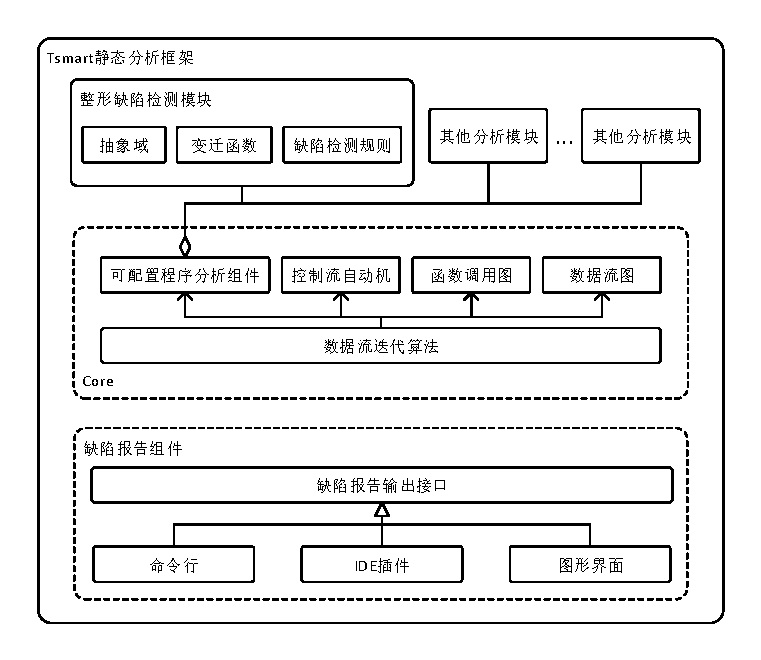
\includegraphics{整型分析_架构图.pdf}
	\caption{整型缺陷分析工具架构图}
	\label{fig:整型分析架构图}
\end{figure}

本模块的实现基于Tsmart静态分析框架,分析框架的输入是C语言源代码,工具的前端程序将C语言代码转化为具有静态单赋值特性的LLVM-IR语言,并在得到的LLVM-IR上构造与之等价的控制流自动机(CFA)。

本模块借助Tsmart提供的接口来获取生成的CFA并以此为基础进行抽象域与检测算法的实现。我们按照前几个小节对理论域RangeInteger、Range、MultiRange、SignRange以及RangeState的介绍,在框架上依次实现其定义及计算规则,同时实现RangeState的状态变迁规则。理论域在工具上的实现结构同图\ref{fig:Domains}。

为了实现整型缺陷检测,我们按照规则\ref{align:overflow}、\ref{align:underflow}和\ref{align:dividebyzero}实现检测规则,并通过调用分析框架提供的缺陷报告输出接口实现整形缺陷的输出。


\section{实验过程与结果}

\subsection{实验设计}

为了客观评价本章提出的整型缺陷检测方法,我们选用Juliet Test Suite测试集作为本工具的检测样本。Juliet测试集由美国国家标准技术研究所 (NIST) 整理出的C语言上包含各类标准错误的样例代码集合。针对每一类定义在CWE上的程序缺陷,Juliet有对应的文件夹包含了在不同情境下出现这类错误的情况。

本次实验选用Juliet测试集中的CWE190\_Integer\_Overflow、CWE191\_Integer\_Underflow和CWe369\_Divide\_by\_Zero三类缺陷样例,其中,CWE190包含7个从测试集s01到s07共3420个测试样例;CWE191包含5个从测试集s01到s05共2622个测试样例;CWE369包含测试集s01、s02共684个测试样例。

Juliet测试集为同种缺陷设计了多种多样的发生环境,包括:不同字节长度、不同符号性(有符号数和无符号数)、结构体、枚举、函数调用、循环等。同时,对应的情景也不尽相同,如套接字应用场景、标准输入输出场景、随机数生成等。

本次实验依次将上述测试集的测试样例作为输入,记录工具对各个样例的测试结果并统计误报率、漏报率以及对应的测试时间。其中,误报是指样例本身无缺陷但测试报告指示存在缺陷的情形,漏报是指样例本身存在缺陷但测试报告指示无缺陷的情形。

实验的运行环境列举如下:
\begin{itemize}
	\item 操作系统:Ubuntu 16.04 LTS 64位版本
	\item 处理器:Intel(R) Core(TM) i7-6500U@2.50GHz 4核心CPU
	\item 内存大小:16GB
\end{itemize}

\subsection{实验结果}

本章介绍的整形缺陷检测工具在Juliet测试集上的测试结果如表\ref{tab:190Result}(CWE190测试结果)、表\ref{tab:191Result}(CWE191测试结果)和表\ref{tab:369Result}(CWE369测试结果)所示:

\begin{longtable}{ccccccc}
	\caption[CWE190测试结果]{CWE190测试结果}
	\label{tab:190Result}  \\ % add \\ command to tell LaTeX to start a new line	
	
	% Appear table header at the first page as well
	\toprule[1.5pt]	
	{\heiti 测试集} & {\heiti 总数} & {\heiti 误报} & {\heiti 漏报} & {\heiti 误报率} & {\heiti 漏报率} & {\heiti 运行时间} \\
	\midrule[1pt]
	\endfirsthead
	
	% Appear the table header at the top of every page
	\multicolumn{7}{c}{续表~\thetable\hskip1em CWE190测试结果}\\
	\toprule[1.5pt]	
	{\heiti 测试集} & {\heiti 总数} & {\heiti 误报} & {\heiti 漏报} & {\heiti 误报率} & {\heiti 漏报率} & {\heiti 运行时间} \\
	\midrule[1pt]
	\endhead 
	
	% Appear \hline at the bottom of every page
	\hline
	\multicolumn{7}{r}{续下页}
	\endfoot 
	\endlastfoot
	
	% data begins here	
	S01	& 418&	11&	0	&0.026315789&	0 & 7m 49s	\\
	S02	&418&	11&	0	&0.026315789&	0 & 7m 37s	\\
	S03	&418&	11&	0	&0.026315789&	0 & 7m 54s	\\
	S04	&418&	11&	0	&0.026315789&	0 & 7m 47s 	\\
	S05	&380&	10&	0	&0.026315789&	0 &	8m 31s	\\
	S06	&684&	18&	0	&0.026315789&	0 &	15m 42s\\
	S07	&684&	18&	0	&0.026315789&	0 &	16m 2s\\
	% more data here
	\bottomrule[1.5pt]
\end{longtable}

\begin{longtable}{ccccccc}
	\caption[CWE191测试结果]{CWE191测试结果}
	\label{tab:191Result}  \\ % add \\ command to tell LaTeX to start a new line	
	
	% Appear table header at the first page as well
	\toprule[1.5pt]	
	{\heiti 测试集} & {\heiti 总数} & {\heiti 误报} & {\heiti 漏报} & {\heiti 误报率} & {\heiti 漏报率}& {\heiti 运行时间}  \\
	\midrule[1pt]
	\endfirsthead
	
	% Appear the table header at the top of every page
	\multicolumn{7}{c}{续表~\thetable\hskip1em CWE191测试结果}\\
	\toprule[1.5pt]	
	{\heiti 测试集} & {\heiti 总数} & {\heiti 误报} & {\heiti 漏报} & {\heiti 误报率} & {\heiti 漏报率}& {\heiti 运行时间}  \\
	\midrule[1pt]
	\endhead 
	
	% Appear \hline at the bottom of every page
	\hline
	\multicolumn{7}{r}{续下页}
	\endfoot 
	\endlastfoot
	
	% data begins here	
	S01	&418	&11	&0	&0.026315789	&0	& 8m 23s	\\
	S02	&418	&11	&0	&0.026315789	&0	& 8m 8s	\\
	S03	&418	&11	&0	&0.026315789	&0	& 8m 50s	\\
	S04	&684	&18	&0	&0.026315789	&0	& 13m 57s	\\
	S05	&684	&18	&0	&0.026315789	&0	& 13m 9s	\\
	% more data here
	\bottomrule[1.5pt]
\end{longtable}

\begin{longtable}{ccccccc}
	\caption[CWE369测试结果]{CWE369测试结果}
	\label{tab:369Result}  \\ % add \\ command to tell LaTeX to start a new line	
	
	% Appear table header at the first page as well
	\toprule[1.5pt]	
	{\heiti 测试集} & {\heiti 总数} & {\heiti 误报} & {\heiti 漏报} & {\heiti 误报率} & {\heiti 漏报率} & {\heiti 运行时间}  \\
	\midrule[1pt]
	\endfirsthead
	
	% Appear the table header at the top of every page
	\multicolumn{7}{c}{续表~\thetable\hskip1em CWE369测试结果}\\
	\toprule[1.5pt]	
	{\heiti 测试集} & {\heiti 总数} & {\heiti 误报} & {\heiti 漏报} & {\heiti 误报率} & {\heiti 漏报率} & {\heiti 运行时间}  \\
	\midrule[1pt]
	\endhead 
	
	% Appear \hline at the bottom of every page
	\hline
	\multicolumn{7}{r}{续下页}
	\endfoot 
	\endlastfoot
	
	% data begins here	
	S01	&418	&11	&0	&0.026315789	&0 & 6m 58s	\\
	S02	&266	&7	&0	&0.026315789	&0	& 4m 35s\\
	% more data here
	\bottomrule[1.5pt]
\end{longtable}

通过表中数据可以看出,本章提出的基于区间运算的整型缺陷分析工具在Juliet-190、191、369上的测试结果良好:误报率小于3\%,漏报率为0\%。其中,造成误报的原因是Tsmart静态分析框架在处理for循环时使用了循环摘要策略,导致整型变量在抽象域上的计算结果有一定的精度丢失。

在分析框架处理循环时,常常需要对循环做摘要处理。这在处理具体问题时是非常有好处的:它避免因循环展开而造成的分析时间不确定的问题,甚至规避了无限次循环展开的情形。为了得到循环摘要,常用的做法是使用循环不变式来计算各个整型变量在循环中的行为,进而计算得到结果。工具的后续研究方向是优化循环不变式的求解,从而获得更高的分析精度。

从分析效率上看,工具在各个测试集上的分析时间均小于10分钟,平均每个测试样例的分析时间小于2秒。具有实际应用价值。

\section{本章小结}

本章介绍了基于区间算数的整型缺陷分析方法,其核心是理论域的设计。本章先介绍了整体的区间设计,随后依次对各个抽象层面进行介绍,并结合控制流自动机,设计了整型变量的缺陷检测规则。最后,在基于Tsmart-V3静态分析框架上做了实现,并通过实验验证了其有效性。

在\ref{sec:Integer}小节,我们介绍了扩展的整数RangeInteger,相比于整数,其具体定义了$ +\infty $和$ -\infty $的概念,同时,我们介绍了有$ -\infty, +\infty $参与的整数运算规则,为后续介绍区间抽象域奠定了基础。在\ref{sec:Range}小节,介绍了基于扩展整数的区间Range,它以单独区间的形式表示了一个整型变量的可能取值范围,并首次定义整数区间上的运算规则。

随后,在\ref{sec:MultiRange}和\ref{sec:SignRange}小节,我们介绍了线性多区间MultiRange与位敏感的线性多区间SignRange,它们的提出分别解决了单独的Range区间精度不足以及无法描述符号性的问题。随后为了进一步提升多区间在区间长度较小时的精度,提出了基于拆分-合并思想的精度提升方法。

最后,结合CPA,提出了基于区间算数的缺陷检测方法。该方法基于区间状态RangeState抽象域,它是CFA上程序状态节点的抽象。通过设计抽象域与变迁规则,可以得到整型变量在程序指令执行前后的取值区间,从而实现整型缺陷分析,并通过实验验证了有效性。

在实验中,测试用例的误报主要原自基于for循环的检测。由于循环摘要的精度受制于循环不变式技术,为了进一步提升整型缺陷分析在循环中的精度,后续的工作重点将集中在循环不变式上。



















































